% styles
\tikzstyle{box} = [draw, text centered, rounded corners]
\tikzstyle{processor} = [box, fill=blue!10]
\tikzstyle{buffer} = [box, fill=red!10]
\tikzstyle{cache} = [box, fill=green!10]

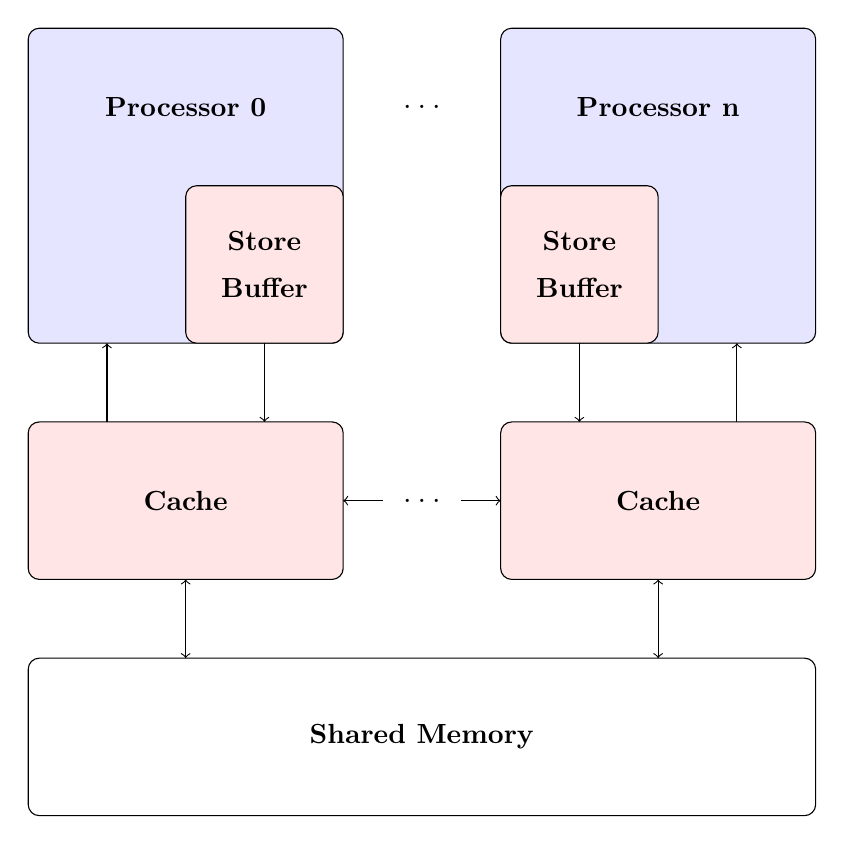
\begin{tikzpicture}

  % \draw[step=1cm,gray,very thin] (-5, 0) grid (5, -10);

  % processors
  \path [processor] (-5, 0) rectangle (-1, -4);
  \path (-3, -1) node (p-0) [] {\textbf{Processor 0}};

  \path [processor] (1, 0) rectangle (5, -4);
  \path (3, -1) node (p-n) [] {\textbf{Processor n}};

  % store buffers
  \path [buffer] (-3, -2) rectangle (-1, -4);
  \path (-2, -2.7) node (s-0) [] {\textbf{Store}};
  \path (-2, -3.3) node (b-0) [] {\textbf{Buffer}};

  \path [buffer] (1, -2) rectangle (3, -4);
  \path (2, -2.7) node (s-n) [] {\textbf{Store}};
  \path (2, -3.3) node (b-n) [] {\textbf{Buffer}};

  % caches
  \path [buffer] (-5, -5) rectangle (-1, -7);
  \path (-3, -6) node (c-0) [] {\textbf{Cache}};

  \path [buffer] (1, -5) rectangle (5, -7);
  \path (3, -6) node (c-n) [] {\textbf{Cache}};

  % heap
  \path [box] (-5, -8) rectangle (5, -10);
  \path (0, -9) node (heap) [] {\textbf{Shared Memory}};

  % arrows
  \path [draw, <-] (-4, -4) -- (-4, -5);
  \path [draw, ->] (-2, -4) -- (-2, -5);
  \path [draw, <->] (-3, -7) -- (-3, -8);

  \path [draw, <-] (4, -4) -- (4, -5);
  \path [draw, ->] (2, -4) -- (2, -5);
  \path [draw, <->] (3, -7) -- (3, -8);

  % \path [draw, <->] (-1, -6) -- (1, -6);
  \path [draw, <-] (-1, -6) -- (-0.5, -6);
  \path (0, -6) node (dots) [] {\large $\ldots$};
  \path [draw, ->] (0.5, -6) -- (1, -6);

  % dots
  \path (0, -1) node (dots) [] {\large $\ldots$};

\end{tikzpicture}
